\documentclass[18pt]{article}

\usepackage[utf8]{inputenc}
\usepackage[T1]{fontenc}
\usepackage{ragged2e}
\usepackage{caladea}
\usepackage{graphicx}
\usepackage{longtable}
\usepackage{wrapfig}
\usepackage{rotating}
\usepackage{epigraph}
\usepackage[normalem]{ulem}
\usepackage{hyperref}
\usepackage{amsmath}
\usepackage{amssymb}
\usepackage{capt-of}
\usepackage{fancyhdr}

\title{
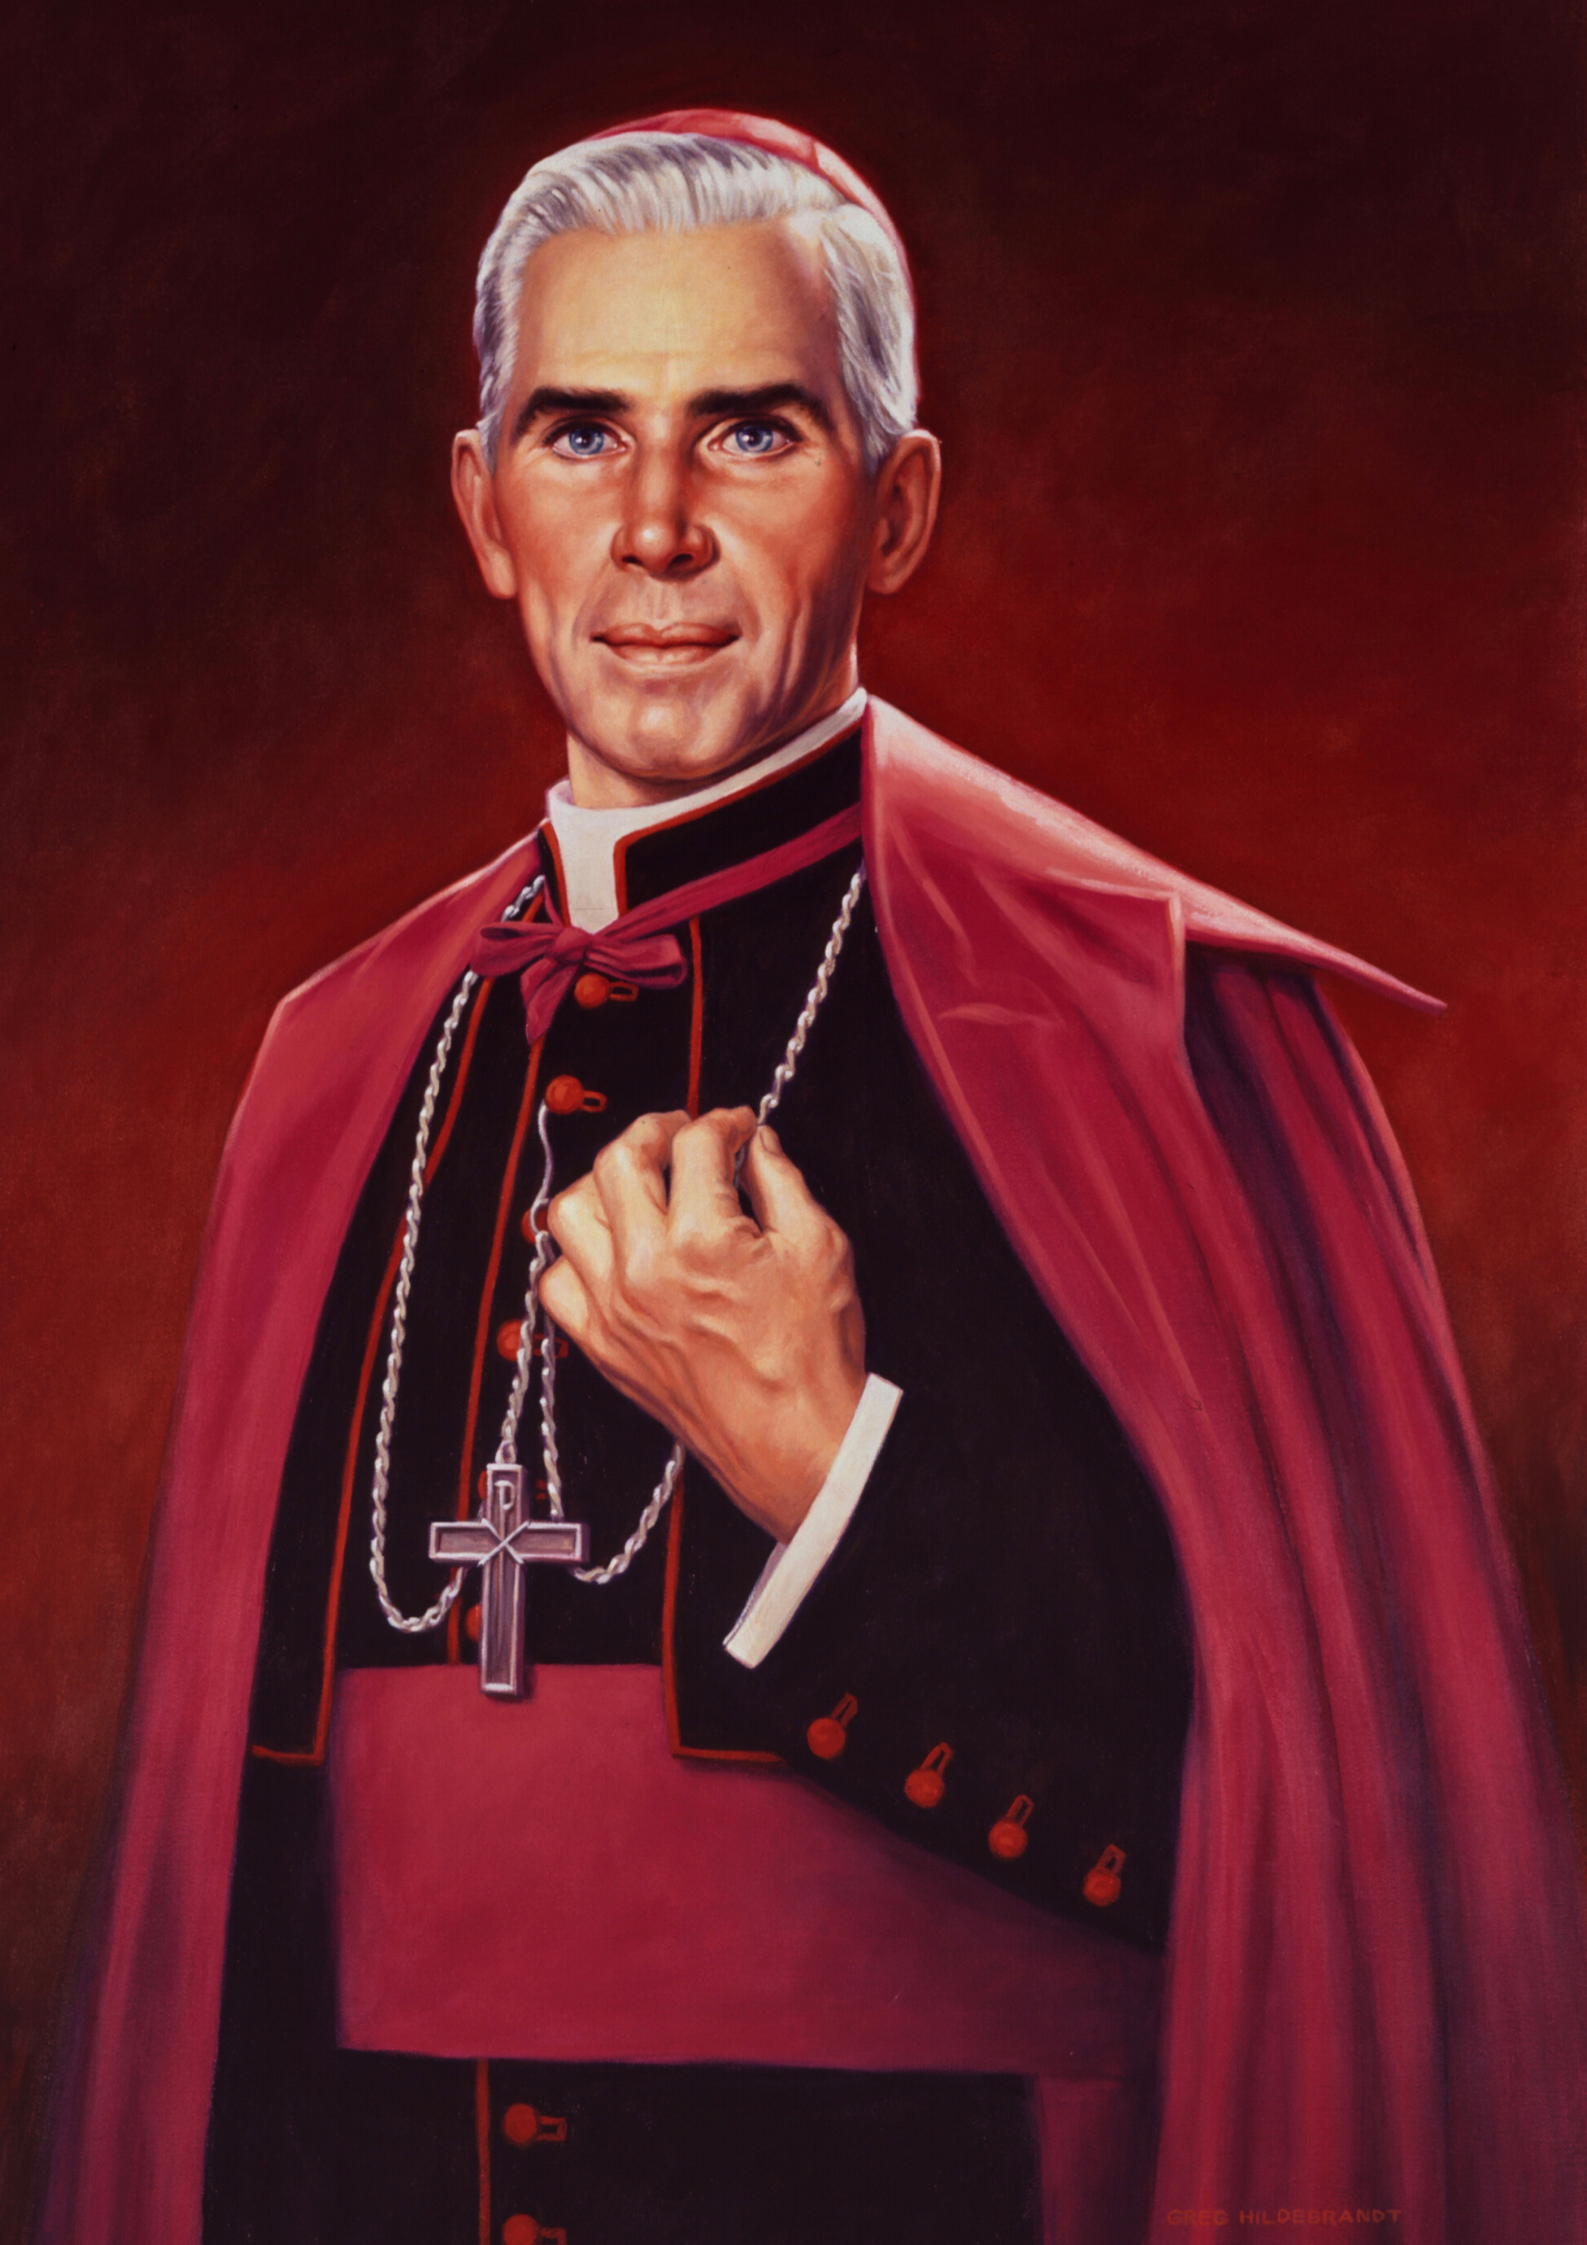
\includegraphics[scale=.35, trim={10cm, 0, 10cm, 0}]{./assets/imagem.jpg}
\par
Novena a São Matias Apóstolo
}

\date{Data de Início: 06/05 \quad Data Litúrgica: 14/05}

\renewcommand{\contentsname}{Sumário}

\begin{document}

\thispagestyle{empty}

\maketitle

\begin{center}
Visite-nos no Telegram: \url{https://t.me/CotidieNovena}
\end{center}

\pagestyle{fancy}
\fancyhf{}
\fancyfoot[LO, CE]{
\includegraphics[scale=0.2]{./assets/cross.png} São Matias Apóstolo, rogai por nós!
}
\fancyfoot[R]{\thepage}

\newpage

\tableofcontents

\newpage

%%%%%%%%%%%%%%%%%%%%%%%%%%%%%%%%%%%%% História %%%%%%%%%%%%%%%%%%%%%%%%%%%%%%%%%%%%%%%%%%%

\begin{justify}
\begin{center}
\section{História}\label{sec:História}
\end{center}


\begin{justify}
\begin{center}
\section{História}\label{sec:História}
\end{center}

\textbf{Nome e eleição}

Matias é nome frequente entre os judeus e quer dizer “dom de Deus”. É o apóstolo que recebeu o dom do grande privilégio de ser agregado aos Doze, tomando o lugar vago deixado pela deserção de Judas Iscariotes. Sua eleição foi mediante sorteio, após a ascensão do Senhor, por proposta de Simão Pedro, que, em poucas palavras, fixou os três requisitos para o ministério apostólico: pertencer aos que seguiam Jesus desde o começo, ser chamado e enviado: “É necessário, pois, que, destes homens que nos acompanharam durante todo o tempo em que o Senhor Jesus viveu no meio de nós, a começar pelo batismo de João até ao dia em que nos foi arrebatado, haja um que se torne conosco testemunha de sua ressurreição”. Essa foi uma das condições necessárias: ser testemunha ocular do Ressuscitado!

\textbf{Testemunha}

Matias esteve, portanto, constantemente próximo de Jesus desde o início até o fim de sua vida pública. Testemunha de Cristo e, mais precisamente, da sua ressurreição, pois a ressurreição do Salvador é a própria razão de ser do cristianismo. Matias, portanto, viveu com os onze o milagre da Páscoa e pôde, com todo o direito, anunciar Cristo ao mundo, como espectador da vida e da obra de Cristo “desde o batismo de João”. Também a segunda e a terceira condições, ser divinamente chamado e enviado, estão claramente expressas pela oração do colégio apostólico: “Senhor, tu que conheces o coração de todos, mostra qual destes dois escolheste”.

\textbf{Sorteio}

A eleição de Matias por sorteio pode causar-nos espanto. Tirar a sorte para conhecer a vontade divina é método muito conhecido na Sagrada Escritura. A própria divisão da Terra Prometida foi mediante sorteio; e os apóstolos julgaram oportuna a conformidade com esse costume. Entre os dois candidatos propostos pela comunidade cristã, José, filho de Sabá, cognominado o Justo, e Matias, a escolha caiu sobre o último. O novo apóstolo, cujo nome brilha na Escritura somente no instante da eleição, viveu com os onze a fulgurante experiência de Pentecostes antes de encaminhar-se, como os outros, pelo mundo afora a anunciar “a glória do Senhor”.

\textbf{Tradição e morte}

Segundo a tradição, Matias evangelizou na Judeia, na Capadócia e, depois, na Etiópia. Ele sofreu perseguições e o martírio, morreu apedrejado e decapitado em Colchis, Jerusalém, testemunhando sua fidelidade a Jesus. Nada se sabe de suas atividades apostólicas, nem se morreu mártir ou de morte natural, pois as narrações a seu respeito pertencem aos escritos apócrifos. À tradição da morte por decapitação com machado liga-se o seu patrocínio especial aos açougueiros e carpinteiros. Normalmente, é representado com um machado ou com uma alabarda, que são símbolos da força do cristianismo e do seu martírio.

\textbf{Relíquias}

Há registros de que Santa Helena, mãe do imperador Constantino, o Grande, mandou trasladar as relíquias de São Matias para Roma, onde uma parte está guardada na igreja de Santa Maria Maior. O restante delas se encontra na antiquíssima igreja de São Matias, em Treves, na Alemanha, cidade que a tradição diz ter sido evangelizada por ele e que o tem como seu padroeiro.

\textbf{Festa}

Sua festa, celebrada por muito tempo a 24 de fevereiro para evitar o período quaresmal, foi fixada pelo novo calendário a 14 de maio, data certamente mais próxima do dia da sua eleição.

\vspace{1em}

\textit{“Ó glorioso Apóstolo, vós sois uma luz em meio à multidão, um testemunho vivo da ressurreição de nosso Senhor. Mesmo sem tê-lo visto, queremos também ser sinais e anunciadores do ressuscitado. Ajuda-nos, mesmo em meio às dificuldades, a evangelizar levando a experiência do encontro pessoal com Jesus!”}

\vspace{1em}

\begin{flushright}
São Matias, rogai por nós!
\end{flushright}

\vfill

\begin{center}
\href{https://santo.cancaonova.com/santo/sao-matias-apostolo-e-martir-testemunho-vivo-da-ressurreicao-de-jesus/}{Fonte: Canção Nova}
\end{center}
\end{justify}

\vfill

\begin{center}
\href{https://catholicnovenaapp.com/saints/about-st-matthias-apostle/}{Fonte: Catholic Novena App}
\end{center}
\end{justify}

%%%%%%%%%%%%%%%%%%%%%%%%%%%%%%%%%%%%% Orações %%%%%%%%%%%%%%%%%%%%%%%%%%%%%%%%%%%%%%%%%%%

\newpage

\begin{center}
\section{Orações}\label{sec:Orações}
\textit{Em nome do Pai, e do Filho, e do Espírito Santo. Amém.}
\end{center}

\subsection*{Oração Inicial}
Ó Deus, que associastes São Matias ao colégio dos Apóstolos, concedei-nos, por sua intercessão, sermos fiéis ao chamado de Cristo e perseverarmos no caminho da fé. Por Cristo, Nosso Senhor. Amém.

\subsection*{Ato de Contrição}
Meu Deus, eu me arrependo de todo o coração de Vos ter ofendido, porque sois infinitamente bom e digno de ser amado sobre todas as coisas. Proponho firmemente, com o auxílio de Vossa graça, não mais pecar. Amém.

\subsection*{Oração Final}
São Matias, fiel seguidor de Cristo, ajudai-me a responder com generosidade ao chamado de Deus, a viver com coragem o Evangelho e a testemunhar o amor de Cristo em minha vida. Intercedei por mim junto ao Senhor para que eu alcance as graças de que tanto necessito, especialmente: (mencionar a graça desejada). Por Cristo, Nosso Senhor. Amém.

\textbf{\textit{Rezar três Pai-Nossos, uma Ave-Maria e um Glória ao Pai em honra à Santíssima Trindade.}}

\textbf{Em nome do Pai, e do Filho, e do Espírito Santo. Amém.}

\vfill

%%%%%%%%%%%%%%%%%%%%%%%%%%%%%%%%%%%%% Orações de Cada Dia %%%%%%%%%%%%%%%%%%%%%%%%%%%%%%%%%%%%%%%%%%%

\newpage

\section*{Orações de Cada Dia}

\subsection*{Primeiro Dia}
São Matias, escolhido entre muitos para ser apóstolo, ajudai-me a reconhecer e valorizar o chamado de Deus em minha vida.

\textit{Concluir com as orações: Ato de Contrição e Oração Final.}

\subsection*{Segundo Dia}
São Matias, testemunha da ressurreição de Cristo, fortalecei minha fé e fazei-me firme na esperança cristã.

\textit{Concluir com as orações: Ato de Contrição e Oração Final.}

\subsection*{Terceiro Dia}
São Matias, que perseverastes na oração com os apóstolos, ensinai-me a buscar sempre a vontade de Deus em tudo.

\textit{Concluir com as orações: Ato de Contrição e Oração Final.}

\subsection*{Quarto Dia}
São Matias, apóstolo missionário, dai-me coragem para anunciar o Evangelho com palavras e ações.

\textit{Concluir com as orações: Ato de Contrição e Oração Final.}

\subsection*{Quinto Dia}
São Matias, fiel até o martírio, ajudai-me a ser firme nas provações e fiel a Cristo até o fim.

\textit{Concluir com as orações: Ato de Contrição e Oração Final.}

\subsection*{Sexto Dia}
São Matias, intercessor junto de Deus, apresentai ao Senhor minhas necessidades e intenções.

\textit{Concluir com as orações: Ato de Contrição e Oração Final.}

\subsection*{Sétimo Dia}
São Matias, exemplo de humildade e serviço, ensinai-me a servir a Deus e aos irmãos com generosidade.

\textit{Concluir com as orações: Ato de Contrição e Oração Final.}

\subsection*{Oitavo Dia}
São Matias, que fostes perseverante na fé, ajudai-me a nunca desanimar diante das dificuldades.

\textit{Concluir com as orações: Ato de Contrição e Oração Final.}

\subsection*{Nono Dia}
São Matias, glorioso apóstolo, alcançai-me a graça de viver e morrer na amizade de Deus, para um dia me unir a vós no Céu.

\textit{Concluir com as orações: Ato de Contrição e Oração Final.}

\vfill

\subsection*{Créditos:}
\href{https://catholicnovenaapp.com/saints/about-st-matthias-apostle/}{Catholic Novena App}

\end{document}
